% ============================================================================
%  Beautified Is Not Forged -- paper v4 (2026-10-14). Built from main.tex (v3) and the v4 drafts: seventeen detectors,
%  threshold-free reading of commercial smoothing, the pre-registered smoothing chain (Addenda 31-36), DF40, fusion
%  (Addendum 37). Every number comes from a results file or FINDINGS.md; tables by make_tables_v4.py (tab_v4_*),
%  make_tables_v3.py, make_tables_cgd.py, make_tables_ali.py; figures by make_fig_*.py. Supplement: supplement_v4.tex.
% ============================================================================
\documentclass[conference]{IEEEtran}
\IEEEoverridecommandlockouts
\usepackage{fontspec}
\setmainfont{texgyretermes}[Extension=.otf,UprightFont=*-regular,BoldFont=*-bold,ItalicFont=*-italic,BoldItalicFont=*-bolditalic]
\usepackage{cite}
\usepackage{amsmath,amssymb,amsfonts}
\usepackage{graphicx}
\usepackage{booktabs}
\usepackage{array}
\usepackage{adjustbox}
\usepackage{xcolor}
\usepackage{url}
\usepackage{capt-of}
\usepackage{algorithm}
\usepackage{algpseudocode}
\usepackage[hidelinks]{hyperref}
\graphicspath{{figs/}}
\newcommand{\ours}{\textsc{Ours}}
\newcommand{\pending}[1]{\textcolor{orange}{[#1]}}
\renewcommand{\dbltopfraction}{0.92}
\renewcommand{\topfraction}{0.92}
\raggedbottom

\begin{document}

\title{Beautified Is Not Forged:\\Measuring and Separating Beautification from Face Forgery}

\author{\IEEEauthorblockN{Qin-Ying Lin, Bo-Rong Chen, Chen-Shan Yu}}

\IEEEaftertitletext{\vspace{-0.6\baselineskip}\begin{center}
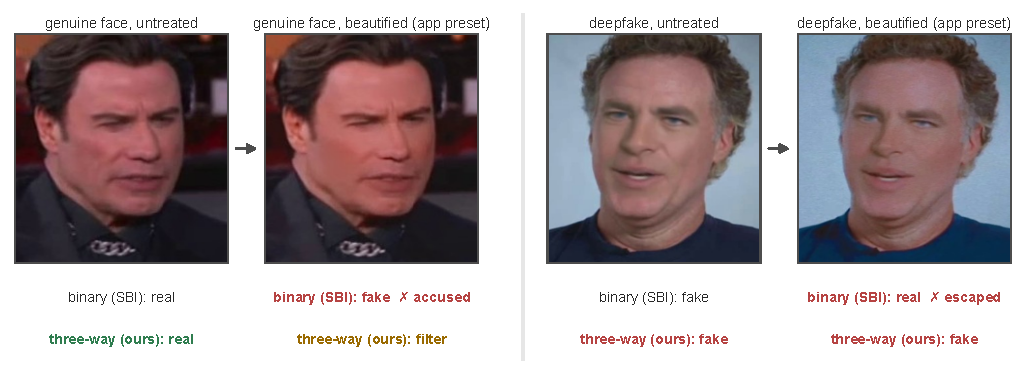
\includegraphics[width=0.92\textwidth]{fig_teaser}
\captionof{figure}{Celeb-DF-B frames of a genuine video and of a deepfake, before and after the same app beautification.
The official SBI checkpoint, at the threshold that accuses 5\% of untreated genuine frames, accuses the beautified genuine
face and lets the beautified deepfake pass. \ours{} calls the first \emph{filter} and the second \emph{fake}. Frames were
chosen where SBI errs after beautification; rates over the benchmark are in Table~\ref{tab:twosided}.}\label{fig:teaser}
\end{center}\vspace{0.2\baselineskip}}
\maketitle


\begin{abstract}
Many of the faces a forgery detector receives have been beautified by a camera app or a retouching service. We measure
what this does to seventeen published detectors with one rule for all of them: the score is the probability of forgery,
the threshold is set on untreated genuine faces, and both errors are counted, genuine faces accused and forgeries let
through; on a retouching service we also read each render against its own original, without a threshold. On three
sources, app presets on Celeb-DF-B, eleven colour filters on Celeb-DF-v2 and sixteen further filters on DFD, every
detector that detects the untreated forgeries loses AUC under app presets; the four CLIP-based detectors of 2025--26
lose 0.08 to 0.12. Fifteen of the seventeen score a genuine face more forged after a retouching service's strongest
skin smoothing in 89--99\% of pairs, and at a threshold that accuses 5\% of the service's untouched originals thirteen
accuse 36--69\% of those faces. A probe of the feature space shows where the damage comes from: a radial luminance
overlay moves a genuine face along the forgery direction three to ten times further than a pure colour look, and the
direction cannot be projected out without losing the forgery evidence itself. A controlled ablation over three seeds
shows that the sign of the error is set in training: a detector shown beautified genuine faces only lets 21 points more
beautified deepfakes through, and a detector shown smoothing on genuine faces only misses every smoothed forgery,
including two smoothing forms it never saw. In pre-registered arms on a LoRA-tuned CLIP model, smoothing in the training
views is necessary and sufficient to stop the accusation of commercially smoothed faces, and a smoothing view that is
class-symmetric is the only recipe that neither accuses smoothed genuine faces nor is fooled by smoothed forgeries, at
a cost of 8--21 points of misses under heavy smoothing and of reenactment detection on DF40; under Effort's tuning
scheme the same view is not sufficient. With beautification on both classes, commercial retouching pairs split into
single operations, and part-level forgeries with exact footprints, a CLIP ViT-L/14 model with LoRA keeps an AUC of
0.87--0.88 under app presets against 0.81 and 0.83 for Effort and Forensics Adapter, is on par with both on untreated
Celeb-DF-v2, DFD and DF40 face swap under each detector's own preprocessing and behind every CLIP detector on DF40
reenactment, accuses 8.6\% of the service's most strongly smoothed faces at the 5\%-FPR rule, and names regions whose
restoration removes 94\% of its detections on held-out part-level forgeries, within a point of the true footprint.
Retrained with the class-symmetric view, this model stops calling smoothed genuine frames forged (35--90\% before,
under 2\% after) and is reported as a variant, because its explanation test fell by 1.4--1.6 points where the
pre-declared limit was 1.0. Seven variants of adversarial training over a measured
beautification operator, a learned inverse, and a decision read from the evidence map did not improve on this; we
report them so that others need not repeat them.
\end{abstract}

% ----------------------------------------------------------------------------
% ----------------------------------------------------------------------------
\section{Introduction}
Face-forgery detectors are used for content moderation, remote identity checks and fact-checking. In these settings a
genuine face called fake accuses a real person, and a forgery called real is let through. Many of the genuine faces such a
detector receives have been beautified. Retouching is common on social media and photo-sharing sites and appears even on
identification documents~\cite{bharati2016}; skin smoothing, whitening, eye enlargement and face slimming are default
options in camera apps and are sold by retouching APIs, and colour presets ship with every photo-sharing app.
Beautification edits the pixels of the face, which is what a forgery detector inspects, but changes neither who is shown
nor what the person does.

We measure both errors on seventeen published detectors, from Xception~\cite{xception}, CADDM~\cite{caddm} and
LAA-Net~\cite{laanet} to the CLIP-based Effort~\cite{effort}, Forensics Adapter~\cite{forensicsadapter},
GenD~\cite{gend2026} and DFD-HR~\cite{dfdhr2026}, with one rule for every detector: the score is its
probability of forgery, the threshold is the one that accuses 5\% of untreated genuine frames, and a forgery not called
fake is a miss whatever else it was called. Three test sources carry beautification that none of the detectors was
trained on. On Celeb-DF-B~\cite{libourel2024}, whose app presets were applied by its authors, re-encoding alone explains
part of the change, so we subtract it; the miss rate still rises by 11.0, 15.2 and 21.8 points for Effort, Forensics
Adapter and SBI~\cite{sbi}. On Celeb-DF-v2 frames under eleven colour filters never used in our training, the AUC of the
two CLIP detectors falls from 0.88--0.89 to 0.81. On DFD frames under sixteen further filters, built after every method
decision of this paper had been taken, it falls from 0.94 to 0.90--0.92 and Effort's miss rate rises by 15 points. The
other direction is as real: fifteen of the seventeen detectors score a genuine face more forged after a retouching
service's strongest skin smoothing in 89--99\% of pairs, and at a threshold that accuses 5\% of the service's untouched
originals thirteen accuse 36--69\% of those faces; several of the rest are near saturation on these stills, so the
threshold hides what the pair statistic shows. The result is specific to skin smoothing: the service's whitening, face
slimming and eye enlarging stay near the 5\% floor for thirteen of the sixteen detectors that are not saturated and
reach at most 17\% for the other three.

Where does the damage come from? In the pooled feature of a CLIP detector trained on FF++ only, the two of eleven
held-out filters that add a radial luminance overlay move a genuine face's forgery logit by $+5.6$ and $+7.8$ on
average, the nine pure colour looks by $+0.1$ to $+2.4$. A luminance ramp around the face reads as a blending boundary,
which is the published mechanism of frame-based detectors~\cite{alphablend2026}. Most of the shift energy of every
held-out filter lies in the subspace spanned by the shifts of beautifications seen in training, and projecting that
subspace out does not help, because the same few directions carry the forgery evidence.

What a detector learns about beautification is therefore set in training, and we test how. With the architecture, data
and recipe held fixed, we vary only which class receives beautified training views. Beautifying genuine faces only, the
recipe a ``filter-robust real class'' would suggest and the direction of fine-tuning on enhanced samples~\cite{saeed2025},
reliably makes beautified deepfakes escape more than showing no beautification at all (21 against 11--17 points of miss
rise, three seeds, two tuning schemes), and when the view is skin smoothing it misses every smoothed forgery: the
detector has learned that smoothing means genuine. Beautifying both classes avoids that, but a view whose form differs
between the classes is learned as a label in the other direction, and we show this in our own recipe and in our main
model. A chain of pre-registered arms on FF++ alone shows that smoothing in the views is necessary and sufficient to
stop an FF++-trained detector from accusing commercially smoothed faces, and that a class-symmetric smoothing view is
the only one that neither accuses nor is fooled, at a stated cost in misses under heavy smoothing and in reenactment
detection. The chain holds for LoRA tuning of CLIP; under Effort's tuning scheme the same view leaves the commercial
renders ranked above their originals. This contradicts the rule of augmenting only the forgery side~\cite{lsda} and
explains the sign of the errors we measure on published detectors.

Our contributions are:
\begin{itemize}
\item \textbf{A two-sided measurement with one rule.} Seventeen detectors on three beautification sources and a
commercial retouching service, scored by the same rule, with video-level confidence intervals, re-encoding separated
from beautification, each baseline also run under its own preprocessing on the video sources, and on the service a
threshold-free reading of each render against its own original.
\item \textbf{The mechanism, measured.} A feature-space probe that quantifies which edits move a CLIP detector toward
``forged'', by how much, and why a linear fix cannot work.
\item \textbf{Exposure decides the sign of the error, and the form of the view is a label too.} A three-arm ablation
over three seeds and two tuning schemes showing that beautification shown to one class is learnt as a label and moves
the errors between misses and false alarms without changing separability; a pre-registered chain on skin smoothing
showing that the view is necessary and sufficient to stop the accusation of commercially smoothed faces, that the
genuine-only recipe is an evasion route, that a class-asymmetric form of the view is learnt as a label in the other
direction, and that a class-symmetric view removes both at a cost in misses under heavy smoothing and in reenactment
detection on DF40.
\item \textbf{A detector and an explanation, with their scope.} With beautification on both classes, commercial
retouching pairs split into single operations and part-level forgeries with exact footprints, a CLIP model with LoRA is
on par with Effort and Forensics Adapter on untreated Celeb-DF-v2, DFD and DF40 face swap, behind them on DF40
reenactment, keeps 0.04--0.07 more AUC under app presets, and names regions whose restoration removes its detections.
It is not a general-purpose reference detector.
\end{itemize}
We also report what did not work, because it bounds the claims: seven variants of adversarial training over a measured
beautification operator, a learned inverse of the edit, and a decision read from the evidence map. A third output class
for beautified faces, which we proposed in an earlier version of this work, does not improve detection either; a detector
with the same data and a single forged output is better by about 0.02 AUC, and the class is kept as a user-facing output.
The main model carries a class-asymmetric smoothing view and calls 35--90\% of whole-crop-smoothed genuine frames
forged; retrained with the symmetric view it calls under 2\% of them forged with no loss of untreated detection, and it
is reported as a variant, not as the main model, because its explanation flip rate fell by more than the pre-declared
1.0 point.

% ----------------------------------------------------------------------------
\section{Related Work}
\textbf{Beautification and forgery detection.} Libourel et al.~\cite{libourel2024} released Celeb-DF-B and measured AUC
drops for three detectors under app presets; Saeed et al.~\cite{saeed2025} show that face enhancement lets deepfakes evade
six detectors and fine-tune on fixed enhanced samples; Concas et al.~\cite{concas2025} report both errors for two CNNs
under a smoothing filter. None trains against the edit, and none scores detectors by a common rule. On a million
smartphone photographs, von Stryk and Keuper~\cite{laionmobile2026} find that the false-alarm rate of a generated-image
detector is set by where its threshold was calibrated, which is why we fix the threshold on untreated genuine faces and
report both errors. The retouching literature labels commercial operations~\cite{retouchingffhq} or restores the
untouched face~\cite{frrffusion,mofrr,reface,wang2019photoshop} without a forgery class; Liu et al.~\cite{miea2026}
attribute forgery and beautification tools in a closed set, and a benchmark of screen-recapture
distortions~\cite{moire2025} names beautification filters as future work.

\textbf{Attacks through natural appearance.} StatAttack~\cite{statattack2023} optimises exposure, blur and noise, and
AdvShadow~\cite{advshadow2024} a shadow overlay, to make forgeries pass; Fatima et al.~\cite{fatima2025} train on the
worst of $K$ random counter-forensic transforms. Adversarial training over semantic perturbations exists for image
classification~\cite{hosseini2018,laidlaw2019,gat2023,ava2021}; its forgery-detection form with a measured
beautification operator does not beat random exposure (Sec.~\ref{sec:negative}).

\textbf{Generalisable forgery detection.} Face X-ray~\cite{facexray} and SBI~\cite{sbi} synthesise blending artefacts
from real images, UCF~\cite{ucf} separates common from method-specific forgery features, LSDA~\cite{lsda} augments the
forgery side of the latent space, and Effort~\cite{effort} and Forensics Adapter~\cite{forensicsadapter} adapt CLIP
ViT-L/14 with few trainable parameters. DeepfakeBench~\cite{deepfakebench} provides common checkpoints and
preprocessing, and DF40~\cite{df40} test sets for forty forgery methods. The alpha-blending
hypothesis~\cite{alphablend2026} holds that frame-based detectors localise compositing artefacts; our measurement that
a luminance ramp around a genuine face raises its forgery score is its benign-edit counterpart.

\textbf{Explanations for detectors.} GAIN~\cite{gain} trains attention so that erasing the attended region removes the
evidence, amortised maskers predict saliency in one pass~\cite{dabkowski2017,phang2020}, and DOLOS~\cite{dolos} compares
methods for localising inpainted regions. We supervise the map with exact footprints and test it by restoring pixels.

% ----------------------------------------------------------------------------
\section{Problem and Evaluation Rule}
\label{sec:protocol}
A face image is \emph{forged} if it shows a person or an action that was not captured: an identity swap, a reenactment, a
synthesised face, or a part replaced by another person's or by generated content. It is \emph{beautified} if its
appearance was edited after capture while identity, expression, pose and speech stay those of the capture: colour and
tone, skin texture, or a smooth reshaping of the person's own features. The two attributes are independent; a beautified
forgery is forged. The tool does not decide: a retouching service that uses a neural network beautifies, and a reenactment
that keeps the identity forges. The supplement lists cases near the boundary. A detector has to return a forgery
score that does not move when a face is beautified; the beautified attribute may be reported separately for the user.

\textbf{One rule for every detector.} Each detector is scored by its probability of forgery. On every source we set the
threshold at a false-alarm rate of 5\% on the untreated genuine frames, keep it fixed, and report under beautification
the false-alarm rate FA (genuine faces called fake) and the miss rate MISS (forgeries not called fake), with the AUC of
untreated and of beautified frames. A forgery that a three-way model sends to its beautified class is a miss; an earlier
version of this work counted only forgeries called \emph{real}, which hid 19.5\% of the beautified Celeb-DF-B deepfakes
that our model sent to the third class, and that rule is withdrawn. Confidence intervals are 95\% percentile intervals
over 1,000 (Celeb-DF-B) or 500 bootstrap resamples of videos; differences between detectors use identical resamples.
Where originals and renders are paired, on the retouching service, we also report the share of renders scored above
their own original and the two medians of the score, which need no threshold.

\textbf{Sources.} Celeb-DF-B~\cite{libourel2024}: 231 Celeb-DF-v2 videos, each as recorded, re-encoded, and beautified
by one of four app presets, for genuine and synthesised faces (32 frames per video). The rise in MISS attributed to
beautification is the rise under the preset minus the rise under re-encoding alone. Celeb-DF-v2 filters: the 516 test
videos of Celeb-DF-v2~\cite{celebdf}, 32 frames each, every frame also saved under one of eleven colour filters from an
open filter library~\cite{pilgram} that no model of ours trained on, assigned per video and applied to the full frame
before the face crop. DFD filters: the 332 DFD videos~\cite{dfd}, 32 frames each, under one of sixteen filters from a
second library, grayscale and sepia, none used in training or in the diagnosis that motivated any design choice; the set
was built after the method was fixed. Commercial retouching: 2,210 FFHQ originals and their renders by a service never
seen in training (Sec.~\ref{sec:measure}). Untreated cross-dataset detection: Celeb-DF-v2 and DFD, each baseline also scored
on the crops of its own training pipeline (dlib, five-point alignment, scale 1.3, 256 px~\cite{deepfakebench}), and the
held-out forgery methods of DF40~\cite{df40} (Sec.~\ref{sec:df40}).

% ----------------------------------------------------------------------------
\begin{figure*}[t]
\centering
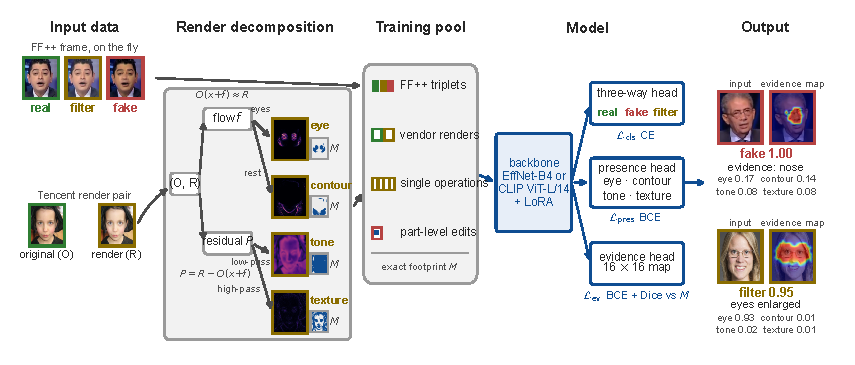
\includegraphics[width=0.86\textwidth]{fig_overview}
\caption{Overview. Each genuine FF++ photograph yields a real / filter / fake triplet on the fly, with beautification
drawn for the genuine and for the forged item; a beautified forgery stays \emph{fake}. Each commercial render $R$ of an
original $O$ is split by optical flow $f$ and photometric residual $P$ into single-operation components with exact
footprints $M$. One backbone feeds the forged and beautified logits, an operation-presence head
and an evidence head trained against $M$. Right: outputs on a held-out part-level forgery and on a render from the unseen
service.}
\label{fig:pipeline}
\end{figure*}

\section{Method}
\label{sec:method}
\subsection{Supervision from paired edits}
\label{sec:data}
Every edited image in our training pool has a pixel-aligned original $x_0$, so the footprint of the edit is known
exactly, $M(x)=\mathrm{dilate}_\rho(\mathbf{1}[\|x-x_0\|_\infty>\tau])$ with $\tau=6$ on 8-bit intensities and $\rho$
the feather width.

\textbf{FF++ triplets.} FF++ c23~\cite{ffpp} under the official 720/140/140 video split. For each genuine training frame
$x_0$ a step draws a genuine item, a beautified item (one of four landmark and skin operations at a random strength, one
of 14 colour filters~\cite{pilgram}, or a random colour grading) and a forged item (a self-blend of $x_0$~\cite{sbi}, an
observed forgery from the four FF++ methods, or a part-level forgery), and the forged item is beautified on top with
probability 0.5. Forged items without landmarks receive the skin smoothing as a whole-crop filter, not as the face-local
operation; Sec.~\ref{sec:mechanism2} shows what this asymmetry teaches. The same random blur or downscale is applied to all three items, so that sharpness does
not predict the label. The FF++-only models of Sec.~\ref{sec:exposure} use nothing else.

\textbf{Commercial renders.} 7,831 FFHQ photographs~\cite{ffhq} and their renders by two retouching services from
RetouchingFFHQ~\cite{retouchingffhq}, Tencent and Megvii, which apply eye enlargement, face lifting, whitening and
smoothing together. Each render $R$ of an original $O$ is split into single-operation components in $O$'s geometry:
dense optical flow~\cite{dis} gives the warp $f$ and a photometric residual $P$, and the components are the eye and
contour warps of $O$ by the masked flow and the low- and high-frequency parts of $P$ added to $O$ (algorithm in the
supplement); applying the four in sequence reproduces $R$ at 108\,dB PSNR. Components whose measured edit falls under the noise floor are dropped, leaving 50,112 of 73,952. The
photometric residual of a render is also added to a self-blend of the same original, so that a measured commercial edit
appears on forged as well as on genuine faces. The third service, Alibaba, is used only for testing.

\textbf{Part-level forgeries.} 61,510 training forgeries on FF++ frames transplant the eyes, nose or mouth of another
identity or regenerate the part with Stable Diffusion inpainting; pixels outside the feathered mask are copied from
$x_0$, so the footprint is exact. The held-out test set uses test-split frames and donors from test videos only.

\subsection{Model}
\label{sec:model}
The detector is a frozen CLIP ViT-L/14~\cite{clip} with rank-16 LoRA~\cite{lora} on every attention projection (3.2\,M
trained parameters of 306\,M). Two linear heads on the pooled feature give the forged logit $z_f$ and the beautified logit
$z_b$; the three-way output is the product of the two Bernoullis, $P(\text{real})=\bar\sigma_f\bar\sigma_b$,
$P(\text{fake})=\sigma_f$, $P(\text{filter})=\bar\sigma_f\sigma_b$, so the forgery score is $\sigma(z_f)$ whatever the
beautified logit says. An operation-presence head and a $1\times1$ convolution on the spatial tokens (the evidence map
$\hat m$, $16\times16$) are trained against the operation labels and the footprints $M$:
\begin{align}
\mathcal{L}={}&\mathrm{BCE}(z_f,y_f)+\mathrm{BCE}(z_b,y_b)+\lambda_s\,\mathbf{1}[y_b]\,\mathrm{BCE}(\hat s,s) \nonumber\\
&+\lambda_m\,\mathbf{1}[M\ \text{exact}]\,\big(\mathrm{BCE}(\hat m,M)+\mathrm{Dice}(\hat m,M)\big),
\label{eq:loss}
\end{align}
with $\lambda_s=\lambda_m=1$. The classifier does not read $\hat m$, so whether the map explains the decision has to be
tested (Sec.~\ref{sec:cgd}). Training: 224\,px crops, AdamW at $10^{-4}$ with warm-up and cosine decay, 8 epochs, a batch
of 16 genuine bases with their forged and beautified items. The checkpoint is chosen on validation data only (FF++
validation macro-F1 for FF++-only models; for full-data models its mean with balanced accuracy on held-out originals and
renders of the training services). No test source is used for any choice. A control with the same data and only the
forged head (``binary'') is trained the same way with validation AUC as the selection rule.

% ----------------------------------------------------------------------------
\section{Results}
\label{sec:results}
\begin{table*}[t]
\centering
\caption{Beautification hurts every detector in both directions: seventeen published detectors and ours under one rule
(score $P(\text{fake})$, threshold at 5\% FPR on untreated genuine frames). Celeb-DF-B: $\Delta$MISS$_\text{beauty}$ is
the rise in misses under the app preset minus the rise under re-encoding alone, FA$_b$ the false-alarm rate on
beautified genuine frames. Celeb-DF-v2 and DFD: eleven and sixteen colour filters never used in training, applied to
the full frame; $\Delta$MISS and $\Delta$FA in percentage points with 95\% video-cluster intervals. LAA-Net is run on
its own crop rebuilt inside ours.}
\label{tab:twosided}
\scriptsize
\begin{adjustbox}{max width=\textwidth}\begin{tabular}{@{}l cccc cccc cccc@{}}
\toprule
 & \multicolumn{4}{c}{Celeb-DF-B (app presets)} & \multicolumn{4}{c}{Celeb-DF-v2 + 11 held-out filters} & \multicolumn{4}{c}{DFD + 16 fresh filters} \\
\cmidrule(lr){2-5}\cmidrule(lr){6-9}\cmidrule(lr){10-13}
Detector & AUC & AUC$_b$ & $\Delta$MISS$_\text{beauty}$ & FA$_b$ & AUC & AUC$_f$ & $\Delta$MISS & $\Delta$FA & AUC & AUC$_f$ & $\Delta$MISS & $\Delta$FA \\
\midrule
Xception & 0.811 & 0.737 & +10.9 [7.4, 14.1] & 5.7 & 0.718 & 0.693 & +1.1 [-1.0, 3.1] & +1.5 [-0.2, 3.2] & 0.854 & 0.834 & +2.0 [-0.6, 5.4] & +2.0 [0.2, 4.3] \\
EfficientNet-B4 & 0.811 & 0.762 & +3.4 [0.9, 5.9] & 7.8 & 0.750 & 0.725 & +2.5 [0.2, 4.8] & +0.8 [-0.3, 2.6] & 0.810 & 0.781 & +6.3 [3.6, 9.2] & -0.5 [-1.9, 1.7] \\
F3Net & 0.798 & 0.731 & +10.9 [7.4, 14.8] & 5.4 & 0.708 & 0.688 & -0.6 [-2.7, 1.6] & +1.3 [-0.8, 3.8] & 0.781 & 0.774 & -8.5 [-11.5, -5.5] & +3.6 [2.1, 5.7] \\
SPSL & 0.781 & 0.727 & +12.4 [9.3, 15.5] & 3.4 & 0.703 & 0.683 & +3.1 [1.5, 4.9] & -0.2 [-1.5, 1.4] & 0.829 & 0.837 & +4.7 [3.2, 6.7] & -1.8 [-2.4, -0.9] \\
UCF & 0.841 & 0.777 & +11.3 [7.6, 15.4] & 5.7 & 0.744 & 0.697 & +3.1 [1.0, 5.5] & +0.9 [-0.6, 2.3] & 0.822 & 0.804 & +5.0 [1.9, 8.0] & +0.3 [-1.6, 2.5] \\
RECCE & 0.785 & 0.723 & +13.8 [10.7, 17.1] & 4.1 & 0.688 & 0.661 & +0.1 [-1.9, 2.0] & +0.9 [-0.8, 2.4] & 0.833 & 0.808 & +7.3 [4.6, 10.7] & -0.2 [-1.7, 1.3] \\
CORE & 0.821 & 0.752 & +13.5 [10.2, 16.6] & 4.0 & 0.715 & 0.693 & -0.0 [-1.5, 1.9] & +0.4 [-0.8, 2.4] & 0.827 & 0.821 & -5.4 [-8.8, -2.9] & +1.6 [-0.3, 3.7] \\
SRM & 0.789 & 0.733 & +15.3 [12.1, 18.7] & 2.8 & 0.717 & 0.712 & -0.1 [-1.4, 1.6] & +0.7 [-0.5, 2.1] & 0.830 & 0.822 & +5.8 [2.4, 9.7] & +0.2 [-1.2, 1.9] \\
SBI~\cite{sbi} & 0.875 & 0.752 & +21.8 [17.3, 26.1] & 1.8 & 0.817 & 0.776 & +8.2 [5.5, 10.4] & -0.6 [-1.5, 0.5] & 0.829 & 0.810 & +4.5 [2.7, 6.3] & +0.4 [-0.7, 1.4] \\
UnivFD & 0.653 & 0.624 & -7.2 [-10.2, -4.9] & 7.6 & 0.662 & 0.622 & -7.2 [-10.6, -4.2] & +7.8 [4.1, 11.7] & 0.840 & 0.801 & -10.2 [-13.5, -6.8] & +11.6 [8.0, 15.7] \\
NPR & 0.503 & 0.498 & -0.7 [-2.2, 0.4] & 3.4 & 0.522 & 0.497 & -38.0 [-43.2, -32.2] & +36.0 [28.7, 43.6] & 0.473 & 0.516 & -13.7 [-20.2, -8.4] & +9.4 [2.4, 15.3] \\
Effort~\cite{effort} & 0.909 & 0.807 & +11.0 [7.7, 14.5] & 5.4 & 0.881 & 0.813 & +23.3 [19.9, 26.3] & -2.8 [-3.7, -1.7] & 0.939 & 0.905 & +15.1 [11.1, 18.6] & -2.3 [-3.1, -1.4] \\
Forensics Adapter~\cite{forensicsadapter} & 0.909 & 0.828 & +15.2 [11.9, 18.6] & 7.9 & 0.887 & 0.814 & +11.9 [8.6, 14.7] & +2.5 [0.3, 5.7] & 0.940 & 0.924 & +8.0 [5.6, 11.2] & -0.6 [-1.6, 0.4] \\
GenD~\cite{gend2026} & 0.924 & 0.807 & +12.0 [8.2, 15.6] & 9.9 & 0.891 & 0.856 & -10.1 [-13.1, -7.1] & +9.9 [7.4, 13.1] & 0.934 & 0.925 & +3.1 [0.7, 5.8] & +1.2 [0.1, 2.2] \\
DFD-HR~\cite{dfdhr2026} & 0.938 & 0.838 & +3.6 [0.6, 6.8] & 14.6 & 0.879 & 0.824 & +8.0 [5.3, 10.5] & +1.6 [0.4, 3.8] & 0.943 & 0.928 & +9.1 [6.8, 11.8] & -2.0 [-2.9, -1.2] \\
CADDM~\cite{caddm} & 0.886 & 0.762 & -2.9 [-5.8, 0.1] & 13.8 & 0.839 & 0.796 & +3.2 [0.7, 5.7] & +3.0 [1.4, 4.7] & 0.845 & 0.818 & +3.8 [2.2, 5.9] & +0.8 [-0.4, 1.9] \\
LAA-Net~\cite{laanet} & 0.889 & 0.698 & +14.7 [10.9, 18.6] & 6.0 & 0.851 & 0.799 & +10.2 [7.4, 12.8] & -0.1 [-1.4, 1.1] & 0.810 & 0.783 & +6.2 [4.2, 7.7] & +0.0 [-0.9, 1.0] \\
\midrule
\ours{}, FF++ only & 0.938 & 0.872 & +7.5 [4.8, 10.5] & 7.8 & 0.898 & 0.851 & -3.5 [-6.1, -1.0] & +7.2 [4.8, 10.9] & 0.943 & 0.932 & -0.3 [-2.5, 2.3] & +3.4 [2.1, 5.1] \\
\ours{} (full data, three-way) & 0.938 & 0.866 & +6.7 [4.0, 9.5] & 9.5 & 0.891 & 0.873 & +7.3 [4.3, 9.9] & -0.4 [-1.4, 0.6] & 0.942 & 0.931 & +8.9 [6.2, 12.1] & -1.0 [-2.4, 0.1] \\
\quad second seed & 0.941 & 0.883 & +8.3 [5.6, 11.0] & 6.7 & 0.887 & 0.875 & +2.0 [-1.1, 4.5] & +0.4 [-1.1, 2.4] & 0.945 & 0.931 & +4.4 [2.2, 7.7] & +0.3 [-0.8, 1.7] \\
\quad symmetric-view variant & 0.941 & 0.868 & +10.0 [7.0, 13.1] & 9.2 & 0.899 & 0.881 & +6.7 [3.9, 9.6] & -0.6 [-1.6, 0.7] & 0.947 & 0.934 & +8.5 [5.7, 12.0] & -0.9 [-2.2, -0.0] \\
same data, forged head only & 0.949 & 0.896 & +7.0 [4.7, 9.0] & 7.4 & 0.914 & 0.883 & +9.8 [7.4, 12.5] & -0.4 [-1.8, 0.9] & 0.961 & 0.952 & +4.2 [2.3, 6.5] & +0.2 [-0.9, 1.4] \\
\bottomrule
\end{tabular}
\end{adjustbox}
\end{table*}

\begin{table}[t]
\centering
\caption{Commercial skin smoothing by a service never seen in training: 2,210 FFHQ originals and their renders at the
strongest of three levels. Share of renders scored above their own original (50 means no signal), medians of
$P(\text{fake})$, and share of renders above the threshold that accuses 5\% of the originals. NPR scores originals and
renders at 1.0. Exposure arms and all renders in Table~\ref{tab:v4tradeoff} and the supplement.}
\label{tab:v4retouch}
\scriptsize
\setlength{\tabcolsep}{3pt}
\begin{adjustbox}{max width=\columnwidth}\begin{tabular}{@{}l ccc@{}}
\toprule
Detector & above own orig.\ (\%) & median $P(\text{fake})$ & above thr.\ (\%) \\
\midrule
Xception & 95.2 & 0.291 $\rightarrow$ 0.944 & 51.6 \\
EfficientNet-B4 & 93.7 & 0.316 $\rightarrow$ 0.964 & 36.3 \\
F3Net & 97.8 & 0.131 $\rightarrow$ 0.974 & 50.6 \\
SPSL & 97.3 & 0.463 $\rightarrow$ 0.963 & 51.2 \\
UCF & 95.4 & 0.031 $\rightarrow$ 0.984 & 41.4 \\
RECCE & 96.5 & 0.120 $\rightarrow$ 0.944 & 36.8 \\
CORE & 96.6 & 0.249 $\rightarrow$ 0.947 & 54.8 \\
SRM & 99.3 & 0.461 $\rightarrow$ 0.668 & 62.8 \\
SBI~\cite{sbi} & 96.2 & 0.208 $\rightarrow$ 0.991 & 37.3 \\
UnivFD & 90.4 & 0.005 $\rightarrow$ 0.019 & 16.6 \\
NPR & n/a & n/a & n/a \\
Effort~\cite{effort} & 95.6 & 0.319 $\rightarrow$ 0.595 & 43.2 \\
Forensics Adapter~\cite{forensicsadapter} & 93.3 & 0.058 $\rightarrow$ 0.354 & 39.7 \\
GenD~\cite{gend2026} & 98.5 & 0.228 $\rightarrow$ 0.921 & 68.7 \\
DFD-HR~\cite{dfdhr2026} & 99.0 & 0.210 $\rightarrow$ 0.711 & 64.9 \\
CADDM~\cite{caddm} & 60.9 & 0.538 $\rightarrow$ 0.745 & 6.3 \\
LAA-Net~\cite{laanet} & 89.2 & 0.234 $\rightarrow$ 0.969 & 17.2 \\
\midrule
\ours{} & 32.5 & 0.002 $\rightarrow$ 0.001 & 8.6 \\
\quad symmetric-view variant & 30.0 & 0.003 $\rightarrow$ 0.001 & 8.1 \\
binary control & 70.5 & 0.000 $\rightarrow$ 0.001 & 9.1 \\
\bottomrule
\end{tabular}
\end{adjustbox}
\end{table}

\subsection{Beautification hurts every detector, in both directions}
\label{sec:measure}
Table~\ref{tab:twosided} scores seventeen published detectors and ours by the rule of Sec.~\ref{sec:protocol}; the
reproduction of each released checkpoint is in the supplement.

\textbf{Commercial retouching.} We begin with the service, where the published detectors fail most and where the
fixed-threshold rule understates the failure. Table~\ref{tab:v4retouch} reads the 2,210 untouched FFHQ originals and
their renders at the strongest skin smoothing (Smoothing-90) in two ways. The first needs no threshold: is the render
scored more forged than its own original, and what are the two medians of $P(\text{fake})$? Fifteen of the seventeen
detectors score the smoothed render above its original in 89--99\% of pairs, and the median moves from 0.21 to 0.99
for SBI, 0.23 to 0.92 for GenD and 0.23 to 0.97 for LAA-Net: a heavily smoothed genuine face is scored like a forgery,
whatever threshold is chosen. The exceptions are NPR, saturated at 1.0, and CADDM
(60.9\% of pairs), which is trained to localise swap artefacts and to suppress identity, so that its evidence is a
boundary cue rather than skin texture.

The second reading is the threshold that accuses 5\% of the service's own originals. Thirteen detectors then accuse
36.3--68.7\% of the Smoothing-90 renders (GenD 68.7\%, DFD-HR 64.9\%); UnivFD, LAA-Net and CADDM accuse 16.6, 17.2 and
6.3\%. This column understates detectors that are near saturation on the service's stills: LAA-Net's threshold is
0.992, so its renders move from a median of 0.23 to 0.97 and still fall under it. The threshold-free column is
therefore the one to read first.
Over all 26,519 renders of the four operations the detectors accuse 5.6--16.8\%, because whitening, face slimming and
eye enlarging at their strongest level stay at 3.7--8.1\% for thirteen of the sixteen detectors other than NPR (Effort reaches
16.8\% on eye enlarging, UnivFD 11.7\% and DFD-HR 9.6\%; supplement): the retouching result is a smoothing result.

Our full-data three-way model accuses 8.6\% of the Smoothing-90 renders (second seed 12.5\%) at the 5\%-FPR rule and
scores the render above its original in 32.5\% of pairs. The binary control trained on the same data gives 9.1\% and
70.5\%, so the third output class is not what removes the accusation. Read by its own three-way output instead, the
main model sends 20.8\% of the untouched originals to its beautified class, and its balanced accuracy on retouched
against untouched faces is 73.5\% (second seed 75.4\%) where the pre-registered target was 75\%, not met as written by
the first seed (supplement).

\textbf{App presets and colour filters.} On Celeb-DF-B every published detector loses AUC under the app presets, most
for those that detect best: SBI from 0.875 to 0.752, Effort from 0.909 to 0.807, Forensics Adapter from 0.909 to 0.828,
GenD from 0.924 to 0.807, DFD-HR from 0.938 to 0.838, CADDM from 0.886 to 0.762 (Libourel et al.~\cite{libourel2024}
report 0.91 to 0.76 for it) and LAA-Net from 0.889 to 0.698, the largest drop of the seventeen. With re-encoding
subtracted, the presets alone raise the miss rate by 21.8 (SBI), 11.0 (Effort), 15.2 (Forensics Adapter), 12.0 (GenD),
3.6 (DFD-HR) and 14.7 (LAA-Net) points; CADDM's loss is a re-encoding loss. The four CLIP detectors of 2025--26 lose
0.08--0.12 AUC, and their errors fall on different sides: DFD-HR and GenD accuse beautified genuine faces (14.6 and
9.9\% against 5\% on untreated frames), Effort and Forensics Adapter let beautified deepfakes through. Under the
Celeb-DF-v2 and DFD colour filters Effort's miss rate rises by 23.3 and 15.1 points [11.1, 18.6] and Forensics
Adapter's by 11.9 and 8.0. A fixed threshold also sees what AUC cannot: our full-data model keeps its AUC under the DFD filters (0.942 to
0.931) while its miss rate rises by 8.9 points, because the filters shift its scores for genuine and forged frames
alike.

\subsection{Where the damage comes from}
\label{sec:mechanism}
For the FF++-only CLIP model, whose forgery decision is a linear head $w$ on the pooled feature, the two held-out
filters with a radial luminance overlay, \emph{earlybird} and \emph{mayfair}, move the forgery logit of a genuine
validation frame by $+7.8$ and $+5.6$ and the nine pure colour looks by $+0.1$ to $+2.4$; the mean shifts of the
overlay filters have cosines of 0.20 and 0.33 with $w$, those of the colour looks 0.00 to 0.09, and forged frames move
far less ($-0.7$ to $+1.8$). A luminance ramp around the face reads as forgery evidence, for a genuine face far more
than for a forged one, which already carries that evidence. For every held-out filter 63--90\% of the shift energy lies
in the subspace spanned by the shifts of training-time beautifications, but projecting that subspace out and refitting
the head fails: removing two directions costs the clean AUC at once (0.987 to 0.933) and the false-alarm rate under the
filters does not fall (17.5--27.5\% against 21.5\%), because the same directions carry the forgery evidence (figure and
per-filter values in the supplement). The separation has to be learnt during training.

\subsection{Exposure decides the sign of the error}
\label{sec:exposure}
With the architecture, data and recipe held fixed, we vary only which class receives beautified training views: none
(P0), genuine faces only (P1), or genuine and forged faces (P2), on three seeds (supplement). P1 is the worst arm on
Celeb-DF-B in every seed: beautified deepfakes escape it 4.5--9.5 points more often than they escape P0 (every paired
interval above zero) and 7.5--11.7 points more often than P2. Beautification shown on genuine faces only is learnt as a
sign of a genuine face. P2 against P0 is $-7.2$, $-4.0$ and $+2.0$ points of miss rise: better on average, within the
seed-to-seed spread of P0 itself (14.0$\pm$3.1 points). On the two colour-filter sources P2 lowers the miss rise by
5--10 points in 9 of 10 seed-by-source cells and raises the false-alarm rise by 2--5 points, while the AUC under the
filters does not change. Exposure therefore moves a detector's beautification errors between misses and false alarms;
it does not make genuine and forged faces more separable. The ordering on Celeb-DF-B replicates when Effort's own
tuning scheme~\cite{effort} replaces LoRA inside the same pipeline ($-4.6$ and $-5.2$ points of miss rise for P2 over
P0 in two seeds, intervals excluding zero); the smoothing remedy of Sec.~\ref{sec:mechanism2} does not. The no-exposure
CLIP model already keeps more AUC under the presets (0.860--0.883) than Effort's released checkpoint (0.807), so most
of the margin of our models over the two CLIP baselines comes from the base recipe rather than from exposure.

\begin{table*}[t]
\centering
\caption{What each training recipe buys and costs; values per seed (seeds 1 / 2 / 3 where trained). Commercial
Smoothing-90 as in Table~\ref{tab:v4retouch}. Smoothed forgery: change of the miss rate on Celeb-DF-v2 forgeries under
the strong whole-crop bilateral filter at the threshold of 5\% FPR on untreated genuine frames; a negative value comes
from accusing every smoothed frame, genuine ones included (see text). Untreated video AUC; Celeb-DF-B under the one rule;
DF40 reenactment video AUC, mean over twelve methods. P0, P1, P2: beautified training views on no class, on genuine
faces only, on both classes. ``--'': not scored.}
\label{tab:v4tradeoff}
\scriptsize
\begin{adjustbox}{max width=\textwidth}\begin{tabular}{@{}l cc c cc cc cc@{}}
\toprule
 & \multicolumn{2}{c}{commercial Smoothing-90} & smoothed forgery & \multicolumn{2}{c}{untreated video AUC} & \multicolumn{2}{c}{Celeb-DF-B} & \multicolumn{2}{c}{DF40 reenactment AUC} \\
\cmidrule(lr){2-3}\cmidrule(lr){5-6}\cmidrule(lr){7-8}\cmidrule(lr){9-10}
Arm & above thr.\ (\%) & above own orig.\ (\%) & miss rise, strong bil. & Celeb-DF-v2 & DFD & AUC$_b$ & $\Delta$MISS$_\text{beauty}$ & FF++ dom. & Celeb-DF dom. \\
\midrule
P0 & 54.2 / 56.1 / 43.5 & 98.5 / 99.0 / 97.0 & -16.0 / -11.8 / +4.3 & 0.938 / 0.938 / 0.940 & 0.981 / 0.979 / 0.978 & 0.860 / 0.883 / 0.883 & +17.0 / +14.2 / +10.8 & 0.906 / 0.877 / 0.873 & 0.692 / 0.720 / 0.633 \\
P2 & 11.7 / 7.1 / 6.9 & 84.1 / 72.4 / 75.5 & -26.5 / -13.3 / -- & 0.917 / 0.920 / 0.935 & 0.973 / 0.975 / 0.972 & 0.879 / 0.893 / 0.877 & +9.8 / +10.3 / +12.8 & 0.809 / 0.785 / -- & 0.644 / 0.643 / -- \\
P2 no smoothing & 55.3 / 67.1 & 98.6 / 99.4 & -28.9 / -33.1 & 0.913 / 0.924 & 0.980 / 0.973 & 0.879 / 0.873 & +12.9 / +12.9 & 0.858 / -- & 0.705 / -- \\
P2 smoothing only & 2.3 / 5.3 & 27.3 / 51.7 & -48.2 / -44.6 & 0.904 / 0.926 & 0.967 / 0.966 & 0.865 / 0.870 & +10.2 / +13.7 & 0.779 / 0.833 & 0.593 / 0.629 \\
P1 & 3.7 / 7.1 / 4.6 & 43.5 / 67.5 / 64.3 & +51.2 / -- / -- & 0.900 / 0.910 / 0.923 & 0.978 / 0.975 / 0.971 & 0.844 / 0.851 / 0.864 & +21.5 / +21.8 / +20.4 & 0.807 / -- / -- & 0.569 / -- / -- \\
P1 smoothing only & 0.7 / 1.0 / 0.9 & 2.6 / 6.5 / 5.4 & +56.4 / +60.0 / +62.9 & 0.922 / 0.929 / 0.939 & 0.974 / 0.977 / 0.964 & 0.887 / 0.896 / 0.893 & +8.6 / +8.5 / +7.3 & 0.871 / 0.869 / 0.900 & 0.673 / 0.689 / 0.679 \\
P2 symmetric smoothing & 5.9 / 6.1 & 53.7 / 51.8 & +14.6 / +17.5 & 0.919 / 0.934 & 0.972 / 0.968 & 0.866 / 0.888 & +14.2 / +10.4 & 0.871 / 0.796 & 0.670 / 0.646 \\
Effort scheme, no beautified views & 56.9 / 63.2 & 99.1 / 99.1 & -32.2 / -- & 0.944 / 0.954 & 0.987 / 0.991 & 0.882 / 0.886 & +10.1 / +10.7 & -- / -- & -- / -- \\
Effort scheme, symmetric smoothing & 14.5 & 88.4 & +24.9 & 0.935 & 0.986 & 0.890 & +10.6 & 0.822 & 0.614 \\
released Effort fine-tuned, no beautified views & 55.3 & 98.5 & -39.9 & 0.926 & 0.976 & 0.805 & +5.8 & -- & -- \\
released Effort fine-tuned, symmetric smoothing & 39.9 & 96.6 & -19.0 & 0.921 & 0.974 & 0.791 & +7.5 & 0.805 & 0.705 \\
\ours{}, three-way, full data & 8.6 / 12.5 & 32.5 / 41.3 & -44.3 / -- & 0.947 / 0.946 & 0.978 / 0.981 & 0.866 / 0.883 & +6.7 / +8.3 & 0.718 / 0.780 & 0.502 / 0.559 \\
\ours{}, symmetric-view variant & 8.1 & 30.0 & +34.1 & 0.954 & 0.983 & 0.868 & +10.0 & 0.738 & 0.539 \\
\ours{}, binary control & 9.1 & 70.5 & -15.0 & 0.956 & 0.987 & 0.896 & +7.0 & 0.842 & 0.647 \\
\bottomrule
\end{tabular}
\end{adjustbox}
\end{table*}

\subsection{Skin smoothing: what an FF++-trained detector learns, and what exposure does to it}
\label{sec:mechanism2}
The retouching result concerns one operation, skin smoothing, and we trace it through a chain of FF++-only arms, each
with its bars written before training (Table~\ref{tab:v4tradeoff}; bars and all numbers per seed and smoothing form in
the supplement). The arms differ only in which class receives beautified training views and in what those views
contain, and no image of any retouching service is used. The scripted smoothing is the same kind of edit as the
service's, a bilateral filter blended inside the face hull at a strength range set to cover two other services, so what
is tested is robustness across implementations and image domains of one operation at matched strength, not
generalisation to an edit the views never contained.

\textbf{No exposure reproduces the published detectors.} P0 accuses 54.2, 56.1 and 43.5\% (three seeds) of the
Smoothing-90 renders and scores the render above its own original in 97--99\% of pairs: the false accusation is what
FF++ training gives by default, and the blur, rescaling and JPEG that P0 applies to both classes do not prevent it.
General beautified views lower the rate to 3.7--7.1\% (P1) and 6.9--11.7\% (P2), but P2 still scores the render above
its original in 72--84\% of pairs.

\textbf{Necessary, and sufficient at a cost.} With smoothing removed from every beautified view of P2 and all other
edits kept, the accusation is 55.3\% [51.9, 58.6] and 67.1\% (two seeds): no other view substitutes for smoothing. With
smoothing as the only view, on both classes, it falls to 2.3\% [1.7, 2.9] and 5.3\% [4.4, 7.0], and the bar on
untreated accuracy is not met as written (Celeb-DF-v2 video AUC 0.904 and 0.926 against 0.938 for P0). Every kind of
beautified view we tried costs 0.01--0.03 there.

\textbf{The genuine-only recipe is an evasion route.} Smoothing shown to genuine faces only lowers the accusation to
0.7--1.0\% (three seeds) and scores the render above its original in only 2.6--6.5\% of pairs. A check written before
any smoothed forgery was scored applies a whole-crop bilateral filter at three strengths and two forms no arm has seen,
a $5\times5$ median filter and a 50\% blend with a Gaussian blur, to Celeb-DF-v2 test frames, at the threshold that
accuses 5\% of untreated genuine frames. The arm then misses every smoothed forgery: its miss rate rises by 56--63
points on the bilateral forms, 38--40 on the median filter and 11--14 on the Gaussian blend. It has learned that
smoothed means genuine. We do not recommend the recipe, and the low accusation rates of the P1 rows are to be read as
this shortcut.

\textbf{The both-class arms carry a shortcut of the opposite sign.} The same test shows a flaw in our own recipe: a
whole-crop bilateral filter on a \emph{genuine} frame is called forged by the main model in 34.9, 79.8 and 90.1\% of
frames at the three strengths and by the smoothing-only both-class arm in 47.8--88.3\%, against 0.8, 16.8 and 39.6\%
for P0. In the training code genuine items receive the face-local smoothing and forged items without landmarks
only the whole-crop filter, so the form of the smoothing predicts the class.

\textbf{A class-symmetric view.} With both forms on both classes, the pre-declared bars were: (a) Smoothing-90 at most
15\% at the 5\%-FPR rule with the render above its original in 25--75\% of pairs; (b) false alarms on smoothed genuine
frames at most 15\% for every form; (c) a miss rise on smoothed forgeries not more than 5 points above P0's for every
form; two seeds. Bars (a) and (b) are met on both seeds: 5.9 and 6.1\%, 53.7 and 51.8\% of pairs, false alarms of
2.2--6.1\%. Bar (c) is not met as written: the miss rises are $+7.6$ to $+20.6$ and exceed P0's by more than 5 points
at the mid and strong strengths, because P0's miss rate \emph{falls} under strong smoothing ($-16.0$ and $-11.8$): P0
accuses everything smoothed (false alarms 39.6 and 42.9\%), which the bar did not anticipate. We keep the bar as
written. Of the arms we trained, the symmetric one alone neither accuses smoothed genuine faces nor is fooled by
smoothed forgeries. Its cost is a miss rise of 8--21 points under smoothing at the fixed threshold and an untreated
Celeb-DF-v2 video AUC of 0.919 and 0.934 against 0.938.

\textbf{Another tuning scheme, and the main model.} Inside Effort's tuning scheme, against that scheme's own reference,
the same view meets bar (b) and not bar (a): Smoothing-90 falls from 56.9 to 14.5\%, but the render is still scored
above its original in 88.4\% of pairs (96.6\% when the released Effort checkpoint is fine-tuned with the view). By the
pre-declared reading the LoRA result stands alone, and the recipe is not scheme-independent. The full-data model
retrained with the symmetric view (one seed) meets the first three conditions of its pre-declared replacement rule:
whole-crop-smoothed genuine frames are called forged in 1.0, 1.6 and 1.7\% of cases, Smoothing-90 is accused at 8.1\%
with the render above its original in 30.0\% of pairs, and untreated video AUC is 0.954 on Celeb-DF-v2 and 0.983 on DFD
(0.947 and 0.978 before). The condition on the explanation test is not met as written: the flip rate is lower by
1.4--1.6 points where the limit was 1.0, with the ceiling falling by the same amount; the fifth, Celeb-DF-B AUC under
the presets, holds (0.868 against 0.866). By the rule the current main model stays, and the retrained model is reported
next to it as the symmetric-view variant.

\subsection{What did not work}
\label{sec:negative}
Three families of methods were tried under pre-registered bars and did not meet them (supplement): adversarial
training over a measured beautification operator, which ends within $\pm$0.01 AUC of random colour grading under
beautification and loses 0.02--0.05 untreated AUC on Celeb-DF-v2; a learned inverse of the edit, which lowers nothing
because a network cannot recover the edit parameters from one image; and a decision pooled from the evidence map, which
halves the false accusations under filters and lets 7.5 points more beautified forgeries through. A third output class
is not a detection contribution: the binary control is about 0.02 AUC better on every source.

\subsection{Untreated forgery detection}
\label{sec:detect}
\begin{table}[t]
\centering
\caption{DF40 held-out, untreated: video AUC, mean over nine face-swap (FS) and twelve reenactment (FR) methods, against
the same-domain real videos. Intervals, every detector and every arm in the supplement.}
\label{tab:v4df40}
\footnotesize
\setlength{\tabcolsep}{3pt}
\begin{adjustbox}{max width=\columnwidth}\begin{tabular}{@{}l cc cc@{}}
\toprule
 & \multicolumn{2}{c}{FF++ domain} & \multicolumn{2}{c}{Celeb-DF domain} \\
\cmidrule(lr){2-3}\cmidrule(lr){4-5}
Detector & FS & FR & FS & FR \\
\midrule
eight CNNs (range) & 0.766--0.860 & 0.754--0.859 & 0.656--0.736 & 0.671--0.740 \\
Effort~\cite{effort} & 0.944 & 0.808 & 0.935 & 0.710 \\
Forensics Adapter~\cite{forensicsadapter} & 0.948 & 0.828 & 0.897 & 0.665 \\
GenD~\cite{gend2026} & 0.966 & 0.935 & 0.947 & 0.828 \\
DFD-HR~\cite{dfdhr2026} & 0.982 & 0.932 & 0.940 & 0.698 \\
CADDM~\cite{caddm} & 0.869 & 0.794 & 0.788 & 0.541 \\
\midrule
\ours{} & 0.952 & 0.718 & 0.905 & 0.502 \\
\quad second seed & 0.960 & 0.780 & 0.928 & 0.559 \\
\quad symmetric-view variant & 0.952 & 0.738 & 0.909 & 0.539 \\
binary control & 0.969 & 0.842 & 0.926 & 0.647 \\
P0 (FF++ only) & 0.981 & 0.906 & 0.925 & 0.692 \\
P2 symmetric smoothing & 0.968 & 0.871 & 0.913 & 0.670 \\
\bottomrule
\end{tabular}
\end{adjustbox}
\end{table}
\textbf{Each detector under its own preprocessing.} Our frames are cropped by one pipeline, while the ten
DeepfakeBench-trained baselines were trained on dlib-aligned 256\,px crops, so each baseline is also scored on crops of
its own pipeline (supplement). Compared each under its own crop, with paired intervals over the common videos, \ours{}
is on par with Effort and Forensics Adapter on untreated Celeb-DF-v2 (frame AUC 0.891; differences $[-0.013, 0.038]$
and $[-0.030, 0.013]$) and DFD (0.942; $[-0.006, 0.025]$ and $[-0.013, 0.017]$); the binary control is 0.914 and 0.967.
Under the app presets \ours{} keeps an AUC of 0.866 and 0.883 (two seeds) against 0.807 and 0.828, and its
beautification-specific miss rise is 6.7 and 8.3 points against 11.0 and 15.2.

\textbf{Forgery methods newer than FF++.}\label{sec:df40} DF40~\cite{df40} adds nine face-swap and twelve reenactment
methods, in an FF++ domain and a Celeb-DF domain. The evaluation was fixed before any
detector was run on it (supplement); no bar was attached and no beautification is applied
(Table~\ref{tab:v4df40}). On face swap the main model is on par with the CLIP detectors: 0.952 in the
FF++ domain against Effort 0.944 and Forensics Adapter 0.948 (paired differences $+0.007$ [$-0.002$, $+0.018$] and
$+0.004$ [$-0.006$, $+0.012$]), and 0.905 in the Celeb-DF domain against 0.935 and 0.897. On reenactment it is behind
every CLIP detector, by 0.090--0.218 in the FF++ domain and 0.163--0.326 in the Celeb-DF domain, every interval below
zero, and at chance in the latter (0.502); the symmetric-view variant is at 0.738 and 0.539. The main model calls
reenactment frames real in 49--51\% and beautified in 21--33\% of cases. A whole-face neural rendering has no blending
boundary and a smooth skin texture, which is what our additions teach the model to read as genuine or beautified. The
scope of the main model is the swap and part-level families it was trained on, under beautification.

\textbf{The loss follows smoothing exposure.} Scored on the same list after the first table was read (post hoc,
nothing selected), the arms of Sec.~\ref{sec:mechanism2} order on FF++-domain reenactment the way they order on
commercial smoothing, in reverse (Table~\ref{tab:v4tradeoff}): P0 0.906 (other seeds 0.877 and 0.873), P2 without
smoothing 0.858, P2 0.809, P2 with smoothing only 0.779, the main model 0.718; the symmetric arm is at 0.871 and 0.796.
In the Celeb-DF domain the three seeds of P0 span 0.633--0.720, so only the larger differences stand out there.
Published detectors show the same trade-off: GenD and DFD-HR are the two strongest on reenactment (0.935 and 0.932)
and, among the CLIP detectors, the two that score a commercially smoothed face above its own original most often (98.5
and 99.0\% of pairs). A detector that reads smooth skin as evidence detects neural rendering and accuses retouching. We
do not claim that this is the only route to reenactment detection, only that every arm of ours and the published
detectors we ran lie on it.

\textbf{Fusion with a boundary-based detector.} CADDM is the one detector that smoothing barely moves, so we fused each
of GenD, DFD-HR, Effort and our P0 with it by the mean, minimum or product of quantile-normalised scores, with released
weights, no training and a reading fixed in advance (supplement). Under the mean rule the accusation of Smoothing-90
renders falls from 43--69\% to 24--29\%, untreated Celeb-DF-v2 video AUC exceeds both members in all four pairs and
FF++-domain reenactment is kept or improved; Celeb-DF-domain reenactment and DFD lose, and no rule meets the three
pre-declared conditions for two published pairs.
Fusion moves the operating point; it is not a way out of the trade-off. Renders are still ranked above their own
originals in 87--92\% of pairs under the mean rule: the fusion lowers the rate at a threshold, not the ordering.

\subsection{Localisation of part-level forgeries}
\label{sec:cgd}
\begin{table*}[t]
\centering
\caption{Explanations on held-out part-level forgeries (FF++ test frames and test-video donors, detected items only).
IoU$_7$: IoU with the exact footprint on a $7\times7$ grid. Flip: share of items that leave \emph{fake} when the named
region, of the same area as the footprint, is restored to the original. Ceil.: the same for the true footprint. Compl.:
the same for the complement. SDXL was never used in training.}
\label{tab:cgd_explain}
\footnotesize
\begin{adjustbox}{max width=\textwidth}\begin{tabular}{l cccc cccc cccc}
\toprule
 & \multicolumn{4}{c}{donor transplant} & \multicolumn{4}{c}{SD-1.5 inpaint} & \multicolumn{4}{c}{SDXL inpaint (unseen editor)} \\
\cmidrule(lr){2-5}\cmidrule(lr){6-9}\cmidrule(lr){10-13}
Map & IoU$_7$ & flip & ceil. & compl. & IoU$_7$ & flip & ceil. & compl. & IoU$_7$ & flip & ceil. & compl. \\
\midrule
centre prior / random region (last col.) & 0.310 & 38.6 & -- & 17.0 & 0.249 & 40.9 & -- & 17.9 & 0.255 & 40.2 & -- & 17.7 \\
\midrule
Score-CAM~\cite{scorecam}, same backbone, no head & 0.408 & 56.5 & 85.8 & 5.9 & 0.334 & 52.4 & 85.2 & 15.4 & 0.341 & 52.4 & 85.9 & 17.1 \\
head, vendor data, no part edits (CLIP) & 0.479 & 78.8 & 89.4 & 2.5 & 0.376 & 53.9 & 69.1 & 14.4 & 0.445 & 68.9 & 78.3 & 8.4 \\
head, part edits, FF++ only (EffNet-B4) & 0.723 & 84.0 & 84.7 & 0.4 & 0.752 & 82.6 & 83.2 & 0.7 & 0.746 & 82.9 & 83.8 & 0.7 \\
\ours{}-lite (EffNet-B4) & 0.807 & 87.9 & 88.0 & 0.0 & 0.820 & 87.4 & 87.6 & 0.4 & 0.812 & 86.9 & 87.2 & 0.4 \\
\textbf{\ours{}} (CLIP ViT-L/14 + LoRA) & 0.834 & 94.0 & 94.1 & 0.1 & 0.841 & 93.6 & 93.7 & 0.4 & 0.831 & 93.5 & 93.6 & 0.3 \\
\bottomrule
\end{tabular}
\end{adjustbox}
\end{table*}
For a detected part-level forgery with footprint $M$, let $\hat A$ be the $|M|$ highest cells of $\hat m$ and
$x_A=x\odot(1-A)+x_0\odot A$ restore a region $A$ to the original. On the three held-out editors the evidence head of
\ours{} reaches IoU$_7$ 0.83--0.84 with the true footprint, and restoring the region it names removes 93.5--94.0\% of
its detections, against 93.6--94.1\% when the true footprint is restored (Table~\ref{tab:cgd_explain}; examples in the supplement); the second seed gives 90.2--90.9\% against 90.2--91.0\%, and the
symmetric-view variant 91.9--92.6\% against 92.0--92.6\% at the same IoU$_7$. Restoring the complement removes at most
0.4\%, a centred region 39--41\% and a random region of equal area 10--16\%. The SDXL editor, not seen in training,
behaves like the others. The named region is therefore sufficient and necessary for the model's own decision on these
forgeries. Post-hoc maps on a backbone without the head reach IoU$_7$ 0.33--0.41 and flips of 52--57\%, and the same
model trained without part-level forgeries 0.38--0.48 and 54--79\%; the footprint supervision carries the result. For
whole-face swaps no method finds a small sufficient region.

% ----------------------------------------------------------------------------
\section{Limitations}
The measurement covers four app presets, 27 colour filters and one retouching service; AR filters that re-render the
face were excluded because their capture pipeline leaks the label. Celeb-DF-v2 under filters is a development source;
Celeb-DF-B and the DFD filters were read once per model. On the retouching service the published detectors were scored
on one shared crop, and eight of the sixteen detectors other than NPR have a 5\%-FPR threshold above 0.96 on its stills, which
is why the threshold-free statistics are reported first. The retouching result is a skin-smoothing result, and the
scripted smoothing in our views is the same kind of edit at a strength range set to cover two other services whose
measurements, like the test service's, existed when the range was set; we claim robustness across implementations and
image domains of that operation, not to an edit the views never contained. The first exposure analysis on the service
was post hoc; the chain that followed it was pre-registered.

The main model carries a class-asymmetric smoothing view and calls 35, 80 and 90\% of whole-crop-smoothed genuine
Celeb-DF-v2 frames forged. The retrained model that removes this exceeded the pre-declared limit on the explanation
test by 0.4--0.6 points and exists for one seed, so it is a variant. The smoothing recipe stands for LoRA tuning of
CLIP alone and costs 8--21 points of misses on smoothed forgeries at the fixed threshold. The gain of both-class over
no exposure under app presets is within seed noise, and our margin over the CLIP baselines under presets is mostly the
base recipe. The main model is behind every CLIP detector on DF40 reenactment and at chance in the Celeb-DF domain;
DF40's real videos are test reals already used in this paper, the scoring of the exposure arms and of CADDM on it is
post hoc, and SBI and LAA-Net are not scored on it.
Separating lightly retouched faces from their originals stays at 73--75\% balanced accuracy on the unseen service, and
the evidence head localises part-level forgeries, not whole-face swaps. The published numbers of Effort and DFD-HR
were not reproduced by us. DFDC and DFDCP are not evaluated, and our DFD set is 332 of its videos, so no DFD number of
ours is comparable to a published one. Inference latency has not been measured (\textit{pending}). A probe of
hand-designed high-frequency statistics (flat skin against edges, face against background, two bands) found no
single-image statistic that separates a commercially smoothed genuine face from a neural-rendered one without also
separating the smoothed face from its own original, and the stills-against-frames difference dominates every
cross-source comparison; the trade-off of Sec.~\ref{sec:df40} has no feature-level handle that we could find.

\section{Conclusion}
Under one rule, beautification makes each of seventeen published face-forgery detectors accuse beautified genuine faces
or let beautified deepfakes through, and fifteen of them score a commercially smoothed genuine face above its own
original in 89--99\% of pairs. The damage has a measurable mechanism, a luminance ramp around the face read as forgery
evidence, and a measurable cause: a detector learns beautification, and the form of a beautified view, as a label of
whichever class it was shown on. For skin smoothing, exposure is necessary and sufficient to stop the accusation, the
genuine-only recipe is an evasion route, and a class-symmetric view avoids both errors under LoRA tuning, at a cost in
misses under heavy smoothing and in reenactment detection. Our full-data model is on par with Effort and Forensics
Adapter on untreated Celeb-DF-v2, DFD and DF40 face swap and behind them on DF40 reenactment, keeps 0.04--0.07 more
AUC under app presets, accuses 8.6\% of the most strongly smoothed commercial renders at the 5\%-FPR rule, and names
the regions its decisions on part-level forgeries depend on. None of the other methods we tried removed the trade-off.

\bibliographystyle{IEEEtran}
\bibliography{refs}
\end{document}
